
\documentclass[
	12pt,				
	oneside,
	a4paper,
	english,
	brazil,
	]{abntex2}

\usepackage{tcc} 								% Customizacoes

% Pacotes fundamentais 
\usepackage{lmodern}								% Fonte Latin Modern
\usepackage[T1]{fontenc}							% Selecao de codigos de fonte.
\usepackage[utf8]{inputenc}						% Codificacao do documento (acentos)
\usepackage{lastpage}							% Usado pela Ficha catalografica
\usepackage{indentfirst}							% Indenta o primeiro paragrafo de cada secao.
\usepackage{color}								% Controle das cores
\usepackage{graphicx}							% Inclusao de graficos
\usepackage{microtype} 							% Melhorias de justificacao
\usepackage[alf,abnt-emphasize=bf]{abntex2cite}	% Citacoes padrao ABNT
\usepackage{lipsum}								% Geracao automatica de textos de exemplo
% ---
	
% Pacotes de citações
\usepackage[brazilian,hyperpageref]{backref}	 
\usepackage[alf]{abntex2cite}					% Citações padrão ABNT

% Informações de dados para CAPA e FOLHA DE ROSTO
\titulo{\Large{o titulo do trabalho}}
\autor{\textbf{Seu nome aqui}}
\local{Salvador (BA)}
\data{2021}

\instituicao{\textbf{Centro Universitário Senai Cimatec}}
\filiacao{ESPECIALIZAÇÃO EM DATA SCIENCE \& ANALYTICS}
\orientador{Seu orientador}

\preambulo{Projeto  apresentado  ao  CENTRO UNIVERSITÁRIO  SENAI  CIMATEC como requisito parcial para obtenção do  título  de  Especialista  em  Data Science \& Analytics.}
% ---

% informações do PDF
\makeatletter
\hypersetup{
     	%pagebackref=true,
		pdftitle={\@title}, 
		pdfauthor={\@author},
    	pdfsubject={\imprimirpreambulo},
	    pdfcreator={LaTeX with abnTeX2},
		pdfkeywords={abnt}{latex}{abntex}{abntex2}{relatório técnico}, 
		bookmarksdepth=4
}
\makeatother
% --- 

% O tamanho do parágrafo é dado por:
\setlength{\parindent}{1.3cm}

% Controle do espaçamento entre um parágrafo e outro:
\setlength{\parskip}{0.2cm}  % tente também \onelineskip

% Compila o índice
\makeindex


% Início do documento
\begin{document}


\selectlanguage{brazil}

% Retira espaço extra obsoleto entre as frases.
\frenchspacing 


% ----------------------------------------------------------
% ELEMENTOS PRÉ-TEXTUAIS
% ----------------------------------------------------------
\pretextual

\imprimircapa
\imprimirfolhaderosto*
\imprimirdeclaracaoisencao

% inserir lista de ilustrações
\pdfbookmark[0]{\listfigurename}{lof}
\listoffigures*
\cleardoublepage
% ---

% inserir lista de tabelas
\pdfbookmark[0]{\listtablename}{lot}
\listoftables*
\cleardoublepage
% ---

% ---
% inserir o sumario
% ---
\pdfbookmark[0]{\contentsname}{toc}
\tableofcontents*
\cleardoublepage
% ---


% ----------------------------------------------------------
% ELEMENTOS TEXTUAIS
% ----------------------------------------------------------
\textual


% ------------------
% ELEMENTOS TEXTUAIS
% ------------------
\textual

\chapter{Introdução}

\lipsum[1-4]
\chapter{Motivação}

\lipsum[1-4]

\cite{Newzoo2019}
\chapter{Objetivo}

\section{Geral}
 
\lipsum[1-2]

\section{Específico}

\lipsum[1-3]


\chapter{Referencial Teórico}

\lipsum[1-2]

\begin{citacao}
\lipsum[1] \cite[p. ~34]{Huizinga2014}
\end{citacao}

\section{Tema 1}

De acordo com \citeonline{SalenZimmerman2012}, ...

\lipsum[4-7]


\section{Tema 2}

De acordo com \citeonline{SalenZimmerman2012}, ...

\lipsum[4-7]

A figura \ref{fig:kings-landing} representa \emph{King's Landing}, cenário da série \emph{Game of Thromes} reproduzido no Minecraft:

\begin{figure}[h]
	\caption{\emph{The King's Landing} no Minecraft}
	\center
	\label{fig:kings-landing}
	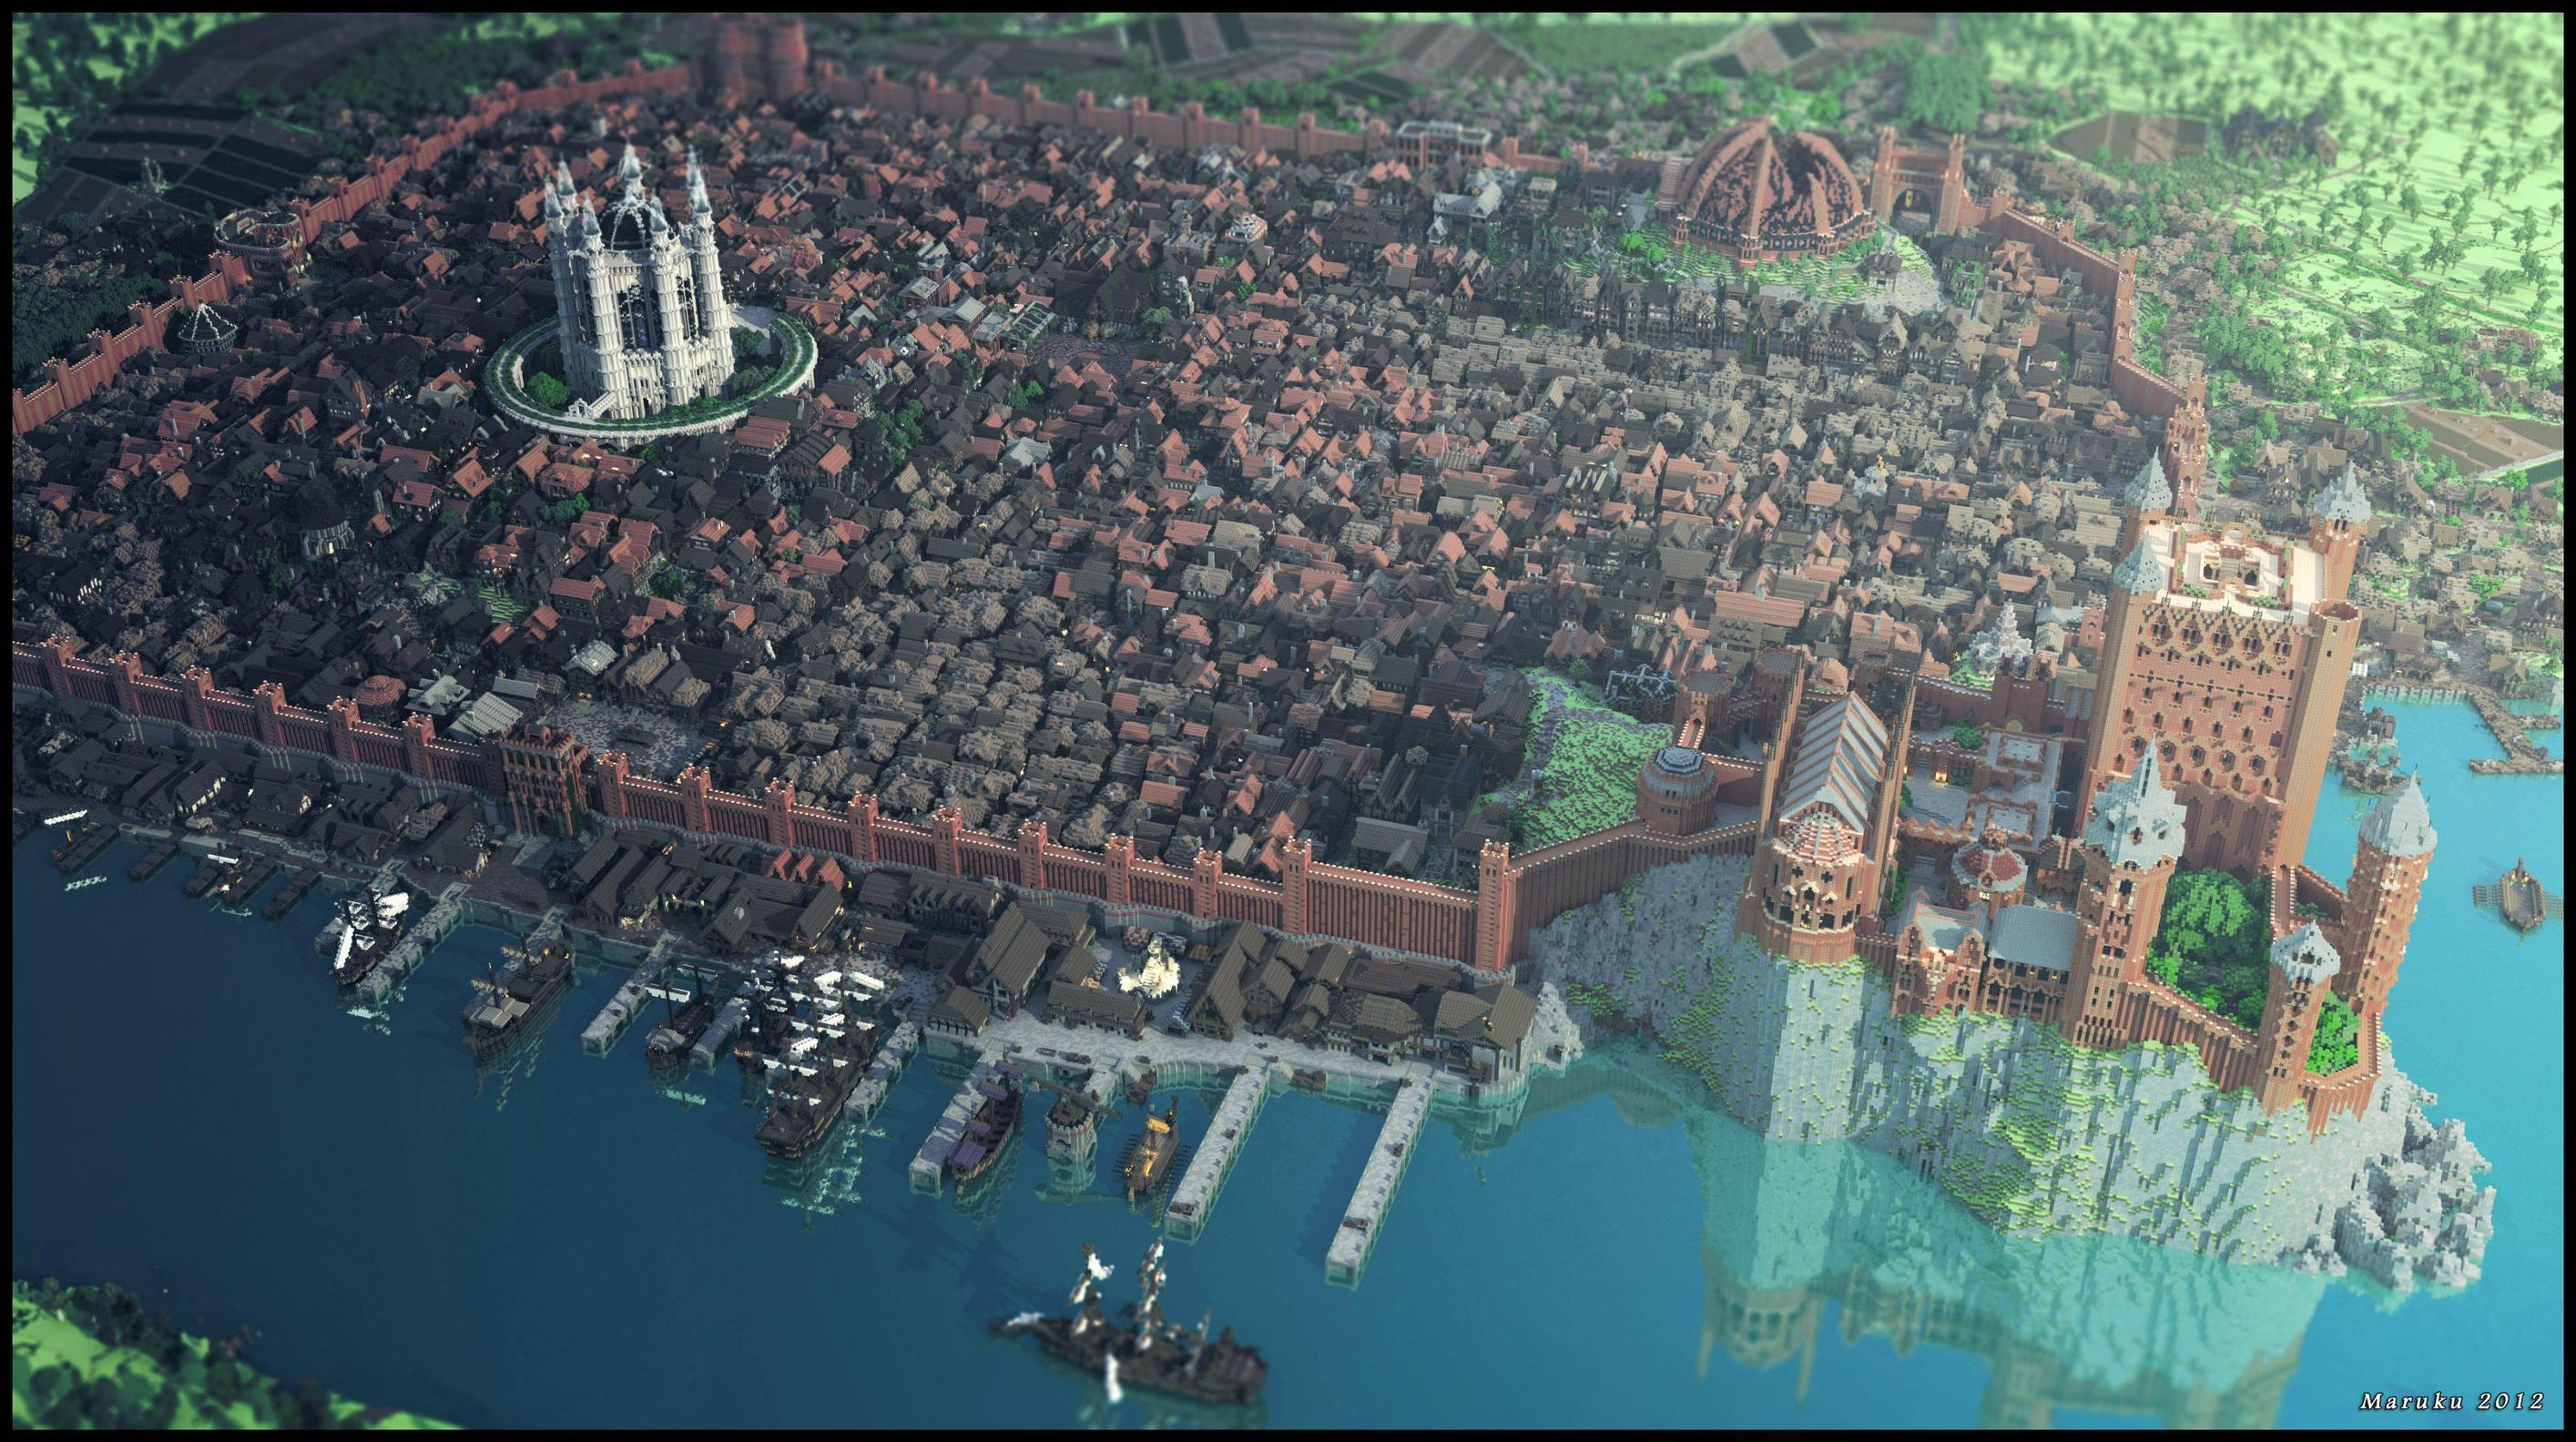
\includegraphics[scale=0.15]{fundamentacao/kings-landing.jpg}
	\fol{Imgur2013}
\end{figure}

\lipsum[10-12]


\chapter{Metodologia}

\lipsum[1-8]


\chapter{Resultados e Discussões}

\lipsum[1-2]

A tabela \ref{tab:newzoo} evidencia os jogos para PC mais populares em junho de 2019:

\begin{table}[h!] 
\caption{Jogos para PC mais Populares - Junho de 2019} 
\label{tab:newzoo}
	\begin{center} 
		\begin{tabular}{|c|l|} 
			\hline POSIÇÃO & JOGO \\
			\hline
			\hline 1 & League of Legends \\ 
			\hline 2 & Minecraft \\ 
			\hline 3 & Counter-Strike: Global Offensive \\
			\hline 4 & Hearthstone: Heroes of Warcraft \\
			\hline 5 & Fortnite \\						
			\hline
		\end{tabular} 
	\end{center}
	\legend{Fonte: \citeonline{Newzoo2019}} 
\end{table}

\lipsum[3-5]
\chapter{Conclusão}

\lipsum[1-4]



% ----------------------------------------------------------
% ELEMENTOS PÓS-TEXTUAIS
% ----------------------------------------------------------
\postextual

% Referências bibliográficas
\bibliography{referencias}

\end{document}
